\documentclass[11pt,a4paper,headsepline]{scrartcl}
\usepackage[utf8]{inputenc}
\usepackage[german]{babel}
\usepackage{amsmath}
\usepackage{amsfonts}
\usepackage{amssymb}
\usepackage{tikz}
\usepackage[left=2cm,right=2cm,top=2cm,bottom=2cm]{geometry}
\usepackage[utf8]{inputenc}
\usepackage{graphicx}
\usepackage{pgfplots}
\usepackage{fancyhdr}
\usepackage{enumerate}
\usepackage{lscape}
\usepackage[scaled]{helvet}

\usetikzlibrary{calc}
\newtheorem{aufgabe}{Aufgabe}


\renewcommand*\familydefault{\sfdefault}
\renewcommand{\arraystretch}{1.1}

\title{\"Ubungen F\"ugetechnik}
\date{}
\makeatletter
\let\Title\@title
\let\Author\@author
\makeatother
\pagestyle{fancy}
\fancyhead[L]{Prof. Dr. Raphael Pfaff}
\fancyhead[R]{86512: Herstellung und Vermarktung}
\fancyfoot[L]{Datei: \jobname}
\fancyfoot[R]{Datum: \today \hspace{.3cm}
\begin{picture}(0,0)(0,0)\put(.5,0){
\includegraphics[height=4cm]{fh_logo}}\end{picture}}

\begin{document}
\vspace{-1cm}
\maketitle
\thispagestyle{fancy}
\pagestyle{fancy}
\vspace{-2cm}



\section*{Schwei{\ss}nahtg\"uteklassen}

\begin{aufgabe}[Sicherheitsbed\"urfnis. Gruppenarbeit 2-3] 
Bewerten Sie die Sicherheitsbed\"urfnisse der Schwei{\ss}n\"ahte der unten in Seitenansicht und Draufsicht gezeigten Kupplung.

\begin{enumerate}[a)]
\item F\"ugen\"ahte Elektrokupplung (Pos. 006) (Kehlnaht a3)
\item Heftn\"ahte Kegel an Kuppelkopf (Pos. 001) (4 x Kehlnaht a4)
\item Verbindung Kuppelkopf-F\"uhrung Elektrokupplung (Pos. 001, 025) (Kehlnaht a4)
\item Verbindung Karabiner-Anschraubplatte (an Pos. 001) (Kehlnaht a3)
\item Fertigungsschwei{\ss}en an Schalenmuffe (Pos. 004)
\item Verbindung Verformungsrohr zu Flansch (Pos. 003) (Steilflankennaht 23mm)
\item F\"ugen\"ahte und Anschraubteile f\"ur HLL-Rohr (an Pos. 001) (Kehlnaht a3)
\item Anlenkteller an Zugstangengeh\"ause (Pos. 002) (V-Naht 15 mm)
\end{enumerate}

\end{aufgabe}
\vspace{.5cm}

%\begin{aufgabe}[Beanspruchungszustand. Gruppenarbeit 2-3] 
%Bewerten Sie die Beanspruchungszust\"ande der Schwei{\ss}n\"ahte der unten in Seitenansicht und Draufsicht gezeigten Kupplung. Bei welchen Schwei{\ss}n\"ahten w\"urden Sie auf eine Berechnung verzichten?
%
%\begin{enumerate}[a)]
%\item F\"ugen\"ahte Elektrokupplung (Pos. 006) (Kehlnaht a3)
%\item Heftn\"ahte Kegel an Kuppelkopf (Pos. 001) (4 x Kehlnaht a4)
%\item Verbindung Kuppelkopf-F\"uhrung Elektrokupplung (Pos. 001, 025) (Kehlnaht a4)
%\item Verbindung Karabiner-Anschraubplatte (an Pos. 001) (Kehlnaht a3)
%\item Fertigungsschwei{\ss}en an Schalenmuffe (Pos. 004)
%\item Verbindung Verformungsrohr zu Flansch (Pos. 003) (Steilflankennaht 23mm)
%\item F\"ugen\"ahte und Anschraubteile f\"ur HLL-Rohr (an Pos. 001) (Kehlnaht a3)
%\item Anlenkteller an Zugstangengeh\"ause (Pos. 002) (V-Naht 15 mm)
%\end{enumerate}
%
%\end{aufgabe}

\begin{aufgabe}[Beanspruchungszustand. Gruppenarbeit 2-3] 
Bewerten Sie die Beanspruchungszust\"ande der Schwei{\ss}n\"ahte der unten in Seitenansicht und Draufsicht gezeigten Kupplung. Bei welchen Schwei{\ss}n\"ahten w\"urden Sie auf eine Berechnung verzichten? Sch\"atzen Sie die wirkenden Kr\"afte ab.

\begin{enumerate}[a)]
\item F\"ugen\"ahte Elektrokupplung (Pos. 006) (Kehlnaht a3)
\item Heftn\"ahte Kegel an Kuppelkopf (Pos. 001) (4 x Kehlnaht a4)
\item Verbindung Kuppelkopf-F\"uhrung Elektrokupplung (Pos. 001, 025) (Kehlnaht a4)
\item Verbindung Karabiner-Anschraubplatte (an Pos. 001) (Kehlnaht a3)
\item Fertigungsschwei{\ss}en an Schalenmuffe (Pos. 004)
\item Verbindung Verformungsrohr zu Flansch (Pos. 003) (Steilflankennaht 23mm)
\item F\"ugen\"ahte und Anschraubteile f\"ur HLL-Rohr (an Pos. 001) (Kehlnaht a3)
\item Anlenkteller an Zugstangengeh\"ause (Pos. 002) (V-Naht 15 mm)
\end{enumerate}

\end{aufgabe}
\vspace{0.5cm}
\begin{aufgabe}[Schwei{\ss}nahtg\"uteklassen und -pr\"ufklassen. Gruppenarbeit 2-3] 
Nehmen Sie f\"ur alle Schwei{\ss}n\"ahte eine geringe Ausnutzung der Festigkeit an. Legen Sie die Schwei{\ss}nahtg\"uteklassen und -pr\"ufklassen fest. \"Uber welche Zertifizierung muss ein Zulieferer verf\"ugen, wenn er diese Teile fertigt?

\begin{enumerate}[a)]
\item F\"ugen\"ahte Elektrokupplung (Pos. 006) (Kehlnaht a3)
\item Heftn\"ahte Kegel an Kuppelkopf (Pos. 001) (4 x Kehlnaht a4)
\item Verbindung Kuppelkopf-F\"uhrung Elektrokupplung (Pos. 001, 025) (Kehlnaht a4)
\item Verbindung Karabiner-Anschraubplatte (an Pos. 001) (Kehlnaht a3)
\item Fertigungsschwei{\ss}en an Schalenmuffe (Pos. 004)
\item Verbindung Verformungsrohr zu Flansch (Pos. 003) (Steilflankennaht 23mm)
\item F\"ugen\"ahte und Anschraubteile f\"ur HLL-Rohr (an Pos. 001) (Kehlnaht a3)
\item Anlenkteller an Zugstangengeh\"ause (Pos. 002) (V-Naht 15 mm)
\end{enumerate}

\end{aufgabe}
\section*{Festigkeitsberechnung}
\begin{aufgabe}[Festigkeitsberechnung] 
Die dynamischen Druck- und Zuglasten auf die Kupplung betragen 200 kN. Bestimmen Sie die Auslastung gem\"a{\ss} DVS 1612 f\"ur folgende Schwei{\ss}n\"ahte:
 \begin{enumerate}[a)]
\item Verbindung Verformungsrohr zu Flansch (Pos. 003)
\begin{itemize}
		\item Steilflankennaht 23mm
		\item 350 mm lang
		\item Verbleibende Badsicherung
		\item \"Ubertr\"agt nur Drucklasten
\end{itemize}
\item Anlenkteller an Zugstangengeh\"ause (Pos. 002)
\begin{itemize}
		\item V-Naht 15mm
		\item durchgeschwei{\ss}t mit Gegenlage
		\item Nahtwinkel 30$^\circ$
		\item 400 mm lang
		\item Verbleibende Badsicherung
		\item \"Ubertr\"agt Zug- und Drucklasten
\end{itemize}

\end{enumerate}
\end{aufgabe}
\newpage
\section*{Schraubenberechnung}

\begin{center}
            		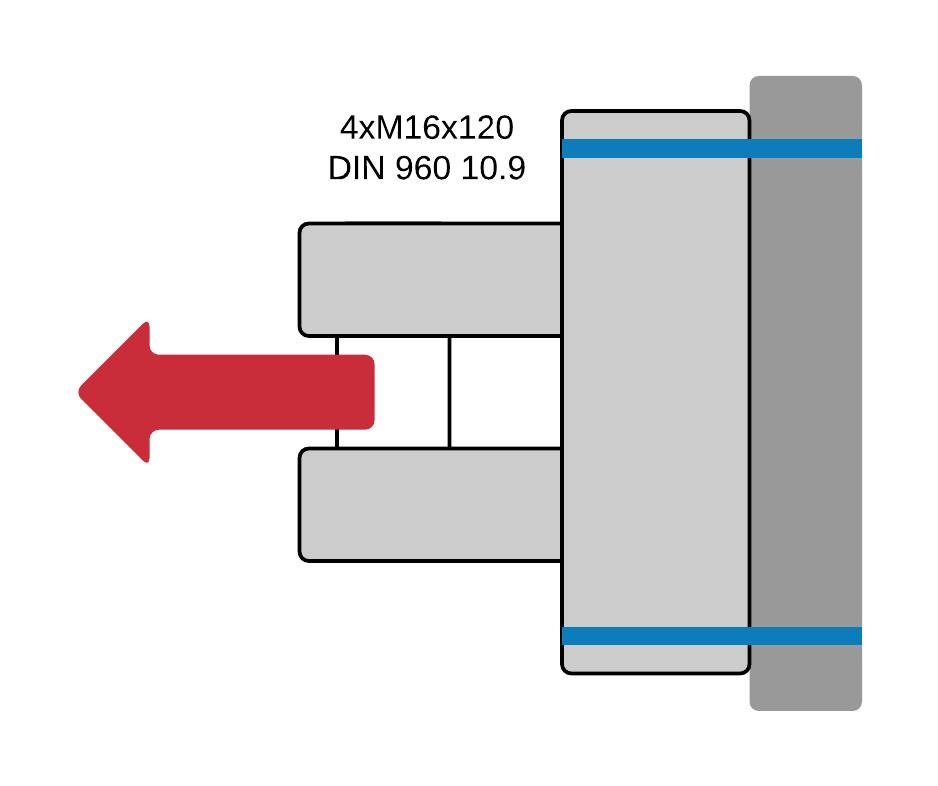
\includegraphics[width=0.38\textwidth]{KonsoleKupplung}
		
        		\end{center}

\begin{aufgabe}[Analytische Schraubenberechnung. Gruppenarbeit 2-3] 

         	
   
Die Schraubenverbindung (Feingewinde) wie im Bild dargestellt wurde mittels ausl\"osendem Drehmomentschl\"ussel nach Sch\"atzung der Reibungsverh\"altnisse montiert. Dabei wurde die maximale Schraubenvorspannung so gew\"ahlt, dass 90 \% der Mindeststreckgenze ausgenutzt werden.

Die verschraubten Teile bestehen aus Stahl, die Montage erfolgt gereinigt. Es sind keine statischen und Setzeffekte zu ber\"ucksichtigen.

Im Feld kommt es zu Querverschiebungen der Konsole und Versagen der Schraubenverbindung durch Querbelastung. Der maximale Auslenkwinkel betr\"agt $\gamma = 15^{\circ}$. 

\begin{enumerate}[a)]
\item Geben Sie die Risikoklasse der Verschraubung an.
\item Bestimmen Sie die minimale und maximale Klemmkraft einer Schraubverbindung unter Ber\"ucksichtigung des Anziehfaktors $\alpha_{A}$.
\item Welche Zugkraft gen\"ugt, um eine Entlastung der Konsole zu bewirken, unter Annahme der ung\"unstigsten Verschraubung. 
\item Welche Zugkraft kann von der dargestellten Verbindung unter Annahme des maximalen Schwenkwinkels \"ubertragen werden ohne eine Querverschiebung zu bewirken?
\end{enumerate}

\end{aufgabe}


\begin{landscape}
\begin{center}
\includegraphics[width = 1.3\textwidth]{DML1}
\newpage
\includegraphics[width = 1.3\textwidth]{DML2}
\end{center}
\includegraphics[width = 1.3\textwidth]{Bauform}
\newpage
\end{landscape}

\includegraphics[width = 0.8\textwidth]{MKJ}
\end{document}